\setcounter{rownumber}{0}
\singlespacing
\chapter{Brillouin-Induced Raman Modes and Device Exploration}
\label{ch:Raman}
\acresetall

\doublespacing

%%%%%%%%%%%%%%%%%%%%%%%%%%%%%%%%%%%%%%%%%%%%%%%%%%%%%%%%%%%%%%%%%%%%

\section{Introduction}
\label{sec:Raman:Introduction}

The overarching goal of this chapter is to explore and demonstrate Brillouin-induced “Raman” modes at room temperature. In other words, we aim to show that acoustic traveling-wave phonons generated by a Brillouin scattering process in a confined medium can organize into discrete standing-wave vibrational modes. This goal represents a convergence of several themes in modern photonics: cavity optomechanics, coherent phonon control, and nonlinear light–matter interactions. Cavity optomechanics has traditionally focused on discrete mechanical resonances (e.g. drumhead membranes or whispering-gallery microresonators) to achieve effects like laser cooling of vibrational modes or phonon lasing. \cite{kippenberg2008cavity, chan2011laser, aspelmeyer2014cavity, vahala2009phonon} In parallel, Brillouin scattering provides a route to manipulate traveling-wave acoustic phonons in extended media, as demonstrated by Brillouin-based laser cooling in optical fiber (a “cavity-less” system). \cite{johnson2023laser, eggleton2013inducing, bahl2012observation, otterstrom2018optomechanical} The research in this chapter aims to bridge these approaches – leveraging traveling-wave SBS in a finite-length system so that the phonons become self-confined, resembling the vibrational modes that give rise to Raman scattering.

This investigation is grounded in the broader context of controlling phonons and light at the mesoscale. High-coherence phonons are garnering interest for precision metrology and quantum information, \cite{balram2016coherent, schliesser2014cavity} spurring new strategies for phonon coherent optomechanical interactions. \cite{kippenberg2008cavity, aspelmeyer2014cavity} Earlier chapters of this dissertation advanced this frontier: Chapter 2 demonstrated the laser cooling of propagating acoustic phonons in an optical fiber, extending optomechanical control to continuous media at room temperature, \cite{johnson2023laser} and Chapter 3 introduced a novel Brillouin spectrometer which offers especially high sensitivity for short (\(<\)\SI{1}{\centi\meter}) lengths over traditional \ac{SBS}. Building on such results, the present work tackles the next challenge: inducing standing-wave acoustic modes in a bulk-like sample through Brillouin processes. Achieving this at room temperature would be significant, as to date strong acoustic mode formation has been mostly limited to cryogenic systems where phonon lifetimes are long. \cite{otterstrom2018optomechanical, galliou2013extremely} By pursuing Brillouin-induced modes under ambient conditions, we push toward practical phonon devices and new regimes of light–sound interaction without the strict need for optical cavities. \cite{pant2011chip}

%--------------------------------------------------------------------%

\section{From Traveling-Wave to Raman-Like Standing-Wave Modes}
\label{sec:Raman:FromTraveling-WavetoRaman-LikeStanding-WaveModes}

\subsection{Review of Brillouin and Raman Scattering}
\label{subsec:Raman:ReviewofBrillouinandRamanScattering}

Brillouin scattering and Raman scattering are two related light–matter interactions that involve inelastic scattering of photons by phonons, but they differ in the nature of the phonons involved. In Brillouin scattering, an incident photon exchanges energy and momentum with a long-wavelength acoustic phonon (a propagating sound wave in the medium). In contrast, Raman scattering typically involves optical phonons or molecular vibrations, which are localized oscillations (e.g. bond vibrations within a molecule or internal lattice vibrations) rather than a continuum acoustic wave. In other words, Brillouin scattering is mediated by traveling acoustic waves in a bulk material, whereas Raman scattering probes standing-wave intramolecular or lattice modes. This fundamental difference is reflected in the frequency scales: acoustic phonons have relatively low frequencies (\si{\giga\hertz} or below) and are responsible for the small Stokes/anti-Stokes shifts in Brillouin spectra, whereas optical phonons and molecular vibrations have much higher frequencies (\si{\tera\hertz}) yielding the larger shifts seen in Raman spectra (see Figure~\ref{fig:Introduction:scattering-domains}). \cite{cardona2007light} It is also reflected in momentum conservation conditions: Brillouin scattering requires phase-matching between the optical wave and an acoustic phonon of a particular wavevector, essentially picking out a traveling phonon mode with a definite momentum. Raman scattering, on the other hand, often involves phonons with near-zero wavevector (e.g. zone-center optical modes in crystals or whole-molecule vibrations) due to the selection rule of crystal momentum conservation in perfect lattices. \cite{ferraro2003introductory}

Despite these distinctions, the line between Brillouin and Raman processes can blur in certain situations. If the medium lacks long-range order or the phonon coherence length is short, the usual momentum-selection rules break down. Shuker and Gammon (1970) \cite{shuker1970raman} showed that in amorphous materials, translational symmetry is lost and essentially all vibrational modes can participate in light scattering. In such cases, even low-frequency acoustic-like modes (normally the realm of Brillouin) become “Raman-active.” This insight explained the observation of broad low-frequency Raman scattering (the so-called boson peak) in glasses by attributing it to acoustic vibrations made allowable by disorder. \cite{duval1990vibrational, winterling1975very, nemanich1977low, martin1974model, malinovsky1986nature, buchenau1986low, malinovsky1987investigation, chumakov2011equivalence} Conversely, in a small or confined system, the vibrational modes are discrete rather than forming a continuous acoustic band. In effect, they approach the molecular limit where each normal mode can scatter light akin to a Raman transition. Thus, one can view Brillouin and Raman scattering as two limits of the same fundamental interaction, distinguished by whether the phonons act as continuous waves or as localized normal modes.

Spatial confinement of acoustic waves can convert the Brillouin regime into a Raman-like regime. In an unbounded or large medium, acoustic phonons exist over a continuum of frequencies and wavevectors (a traveling-wave picture). But if the medium is bounded (e.g., a micron-scale particle or a cavity of finite length) the acoustic field must satisfy boundary conditions, leading to a set of allowed eigenmodes. Classic elasticity theory by Lamb (1882) \cite{lamb1881vibrations} provided the first analysis of this: a homogeneous elastic sphere supports only certain quantized vibration modes (classified into spheroidal and torsional families) dictated by the sphere’s finite size and free-surface boundary condition. These quantized vibration modes are true standing-wave modes confined to the sphere. Subsequent work extended Lamb’s theory to include various effects such as surface tension and clamping for small particles, \cite{} but the essential result is that a finite object has discrete acoustic eigenmodes. Experimentally, Duval et al. (1986) \cite{duval1986vibration} performed a notable demonstration by observing very-low-frequency Raman scattering from nanometer-sized microcrystals embedded in glass. The Raman spectra showed distinct peaks whose frequencies scaled inversely with the particle diameter, exactly as expected for Lamb’s vibrational modes in a sphere. Duval identified these peaks as the confined acoustic eigenmodes (“particle vibrational modes”) of the microcrystallites, which had become Raman-active. This exemplified how a Brillouin-like acoustic wave (here, a sphere’s breathing or shear wave) can become Raman-like when spatially confined. When an acoustic phonon is restricted by boundaries, it is no longer a freely propagating wave but rather a normal mode with a discrete frequency – effectively turning a Brillouin interaction into a Raman-style interaction with a set of allowed modes.

% Conceptual illustration of the transition from a traveling acoustic wave to standing-wave vibrational modes. In a bulk material (left), light scatters from a continuum of acoustic waves (Brillouin scattering), whereas in a confined medium (right), only discrete phonon modes are allowed, producing Raman-like spectral lines. Spatial confinement and acoustic reflections thus shift the scattering from the Brillouin regime toward a Raman-like regime.

Contemporary research in cavity optomechanics and related fields has leveraged this wave-to-mode transition as well. For instance, Renninger et al. (2018) \cite{renninger2018bulk} showed that by shaping the geometry of a \si{\centi\meter}-scale crystal, one can support long-lived acoustic standing-waves even in a bulk solid. At low temperature, the phonon coherence length in their system exceeded the system size, and the crystal effectively behaved as a giant “phonon cavity” with high-Q (quality) acoustic modes. \cite{renninger2018bulk, maccabe2020nano} These modes were accessed via Brillouin interactions, blurring the line between traditional Brillouin and Raman: the process was Brillouin in origin (photoelastic coupling to sound waves) but the phonons were in discrete cavity modes like Raman vibrations. These studies underscore that confined acoustic phonons can take on the character of Raman modes.

\subsection{Brillouin-Induced Raman Modes}
\label{subsec:Raman:Brillouin-InducedRamanModes}

In a traditional SBS experiment, a pump laser drives an acoustic wave through electrostriction, and the scattered Stokes light is down-shifted by the acoustic frequency \(f_{\rm B}\). In an unbounded or long medium, \(f_{\rm B}\) is determined by material properties (sound speed and optical dispersion) and the acoustic wave can be thought of as a traveling grating moving through the medium. If the medium is shortened such that the acoustic wave can reflect off the sample boundaries, the traveling acoustic wave can auto-interfere with itself to form a standing-wave pattern in the medium. Under these system conditions, a phonon induced by \ac{SBS} will propagate to the sample end, reflect (assuming a high acoustic impedance mismatch at the boundary), and traverse the medium in the reverse direction. If the length \(L\) between acoustic interfaces is a half-integer number of acoustic wavelengths, the forward and backward phonon waves can interfere to form a standing wave pattern (i.e., a resonance), in essence trapping the traveling phonon in the cavity defined by the sample. This standing wave in turn acts like a stable grating, enhancing the scattering of light at well-defined frequencies corresponding to its resonances. We term these resonant phonon excitations “Brillouin-induced Raman modes” to reflect their hybrid character.

In more concrete terms, the finite-length system behaves like an acoustic Fabry–Pérot cavity. For a longitudinal acoustic mode, the condition for a standing wave is that an integer number \(n\) of half-wavelengths equals the round-trip length: \(n \cdot (\lambda_{\rm s}/2) = L\). Equivalently, the allowed acoustic frequencies are

\begin{equation}
f_{\rm n} = \frac{n\,v_{\rm s}}{2L},
\end{equation}

where \(v_{\rm s}\) is the sound velocity in the medium and \(n = 1, 2, 3, \dots\) indexes the mode order. The lowest-frequency mode (\(n = 1\)) has a fundamental frequency \(f_{\rm 1} \approx v_{\rm s}/(2L)\), and higher modes are integer multiples of this fundamental (assuming a simple one-dimensional confinement). Thus, instead of a single Brillouin shift \(f_{\rm B}\), one expects a ladder of equally spaced phonon modes in the scattering spectrum, resembling a Raman vibrational progression. The spacing \(\Delta f\) between adjacent modes is approximately \(\Delta f \approx v_{\rm s}/(2L)\), set solely by the cavity length and sound speed. For example, if \(L =\) \SI{10}{\milli\meter} in a medium where \(v_{\rm s} =\) \SI{5000}{\meter\per\second}, the fundamental mode would be \(f_{\rm 1} \sim\) \SI{250}{\kilo\hertz} and overtones at \SI{500}{\kilo\hertz}, \SI{750}{\kilo\hertz}, etc. In principle, a sufficiently short and high-Q acoustic cavity could produce a comb of multiple \si{\giga\hertz}-range lines (analogous to molecular vibrational Raman lines) out of what would ordinarily be a single broad Brillouin gain peak.

These Brillouin-induced modes would manifest as distinct peaks in the spectrum of the scattered light. In addition to the usual broadened Brillouin spectrum (with width given by acoustic damping), one would see a series of sharp lines at \(f_{\rm 1}, f_{\rm 2}, f_{\rm 3}, \dots\) around the center scattered frequency. Such a spectrum would be clear evidence that the phonon field is not only a freely propagating wave but also oscillating in discrete standing patterns (i.e., an optically driven acoustic resonator within the material). This is conceptually similar to stimulated Raman scattering in a molecule, where one can get a cascade of Stokes lines corresponding to \(1\hbar\omega_{\rm vib}\), \(2\hbar\omega_{\rm vib}\), \(3\hbar\omega_{\rm vib}\) energy shifts if the pump is intense. Here the “molecular vibration” is replaced by an acoustic cavity mode. If the pump power is high enough to drive the acoustic mode into the nonlinear regime, one might even observe multiple orders of Stokes (and anti-Stokes) as the phonon population builds up in those modes.

The idea of \ac{SBS}-driven acoustic modes has parallels in prior work. In the cryogenic experiment of Renninger et al. mentioned earlier, \cite{renninger2018bulk} a bulk acoustic mode was driven via Brillouin scattering in a \si{\centi\meter}-scale quartz crystal. At low temperatures, they observed ultra-narrow acoustic resonances (indicative of discrete modes) in place of a broad Brillouin response, confirming that acoustic coherence across the entire sample can indeed produce a modal spectrum. In our case, we seek to do this at room temperature by engineering a shorter effective acoustic cavity. We aim to accomplish this by taking advantage of our Coherently Stimulated Brillouin Spectrometer (\ac{CoBS}), which offers \(\sim 10^6\) improvement in scattered power for \(\sim\)\si{\centi\meter} lengths over traditional \ac{SBS} (see Appendix~\ref{appendix:comparison} for a comparison of scattered powers across Brillouin techniques).

\begin{figure}[t]
  \centering
  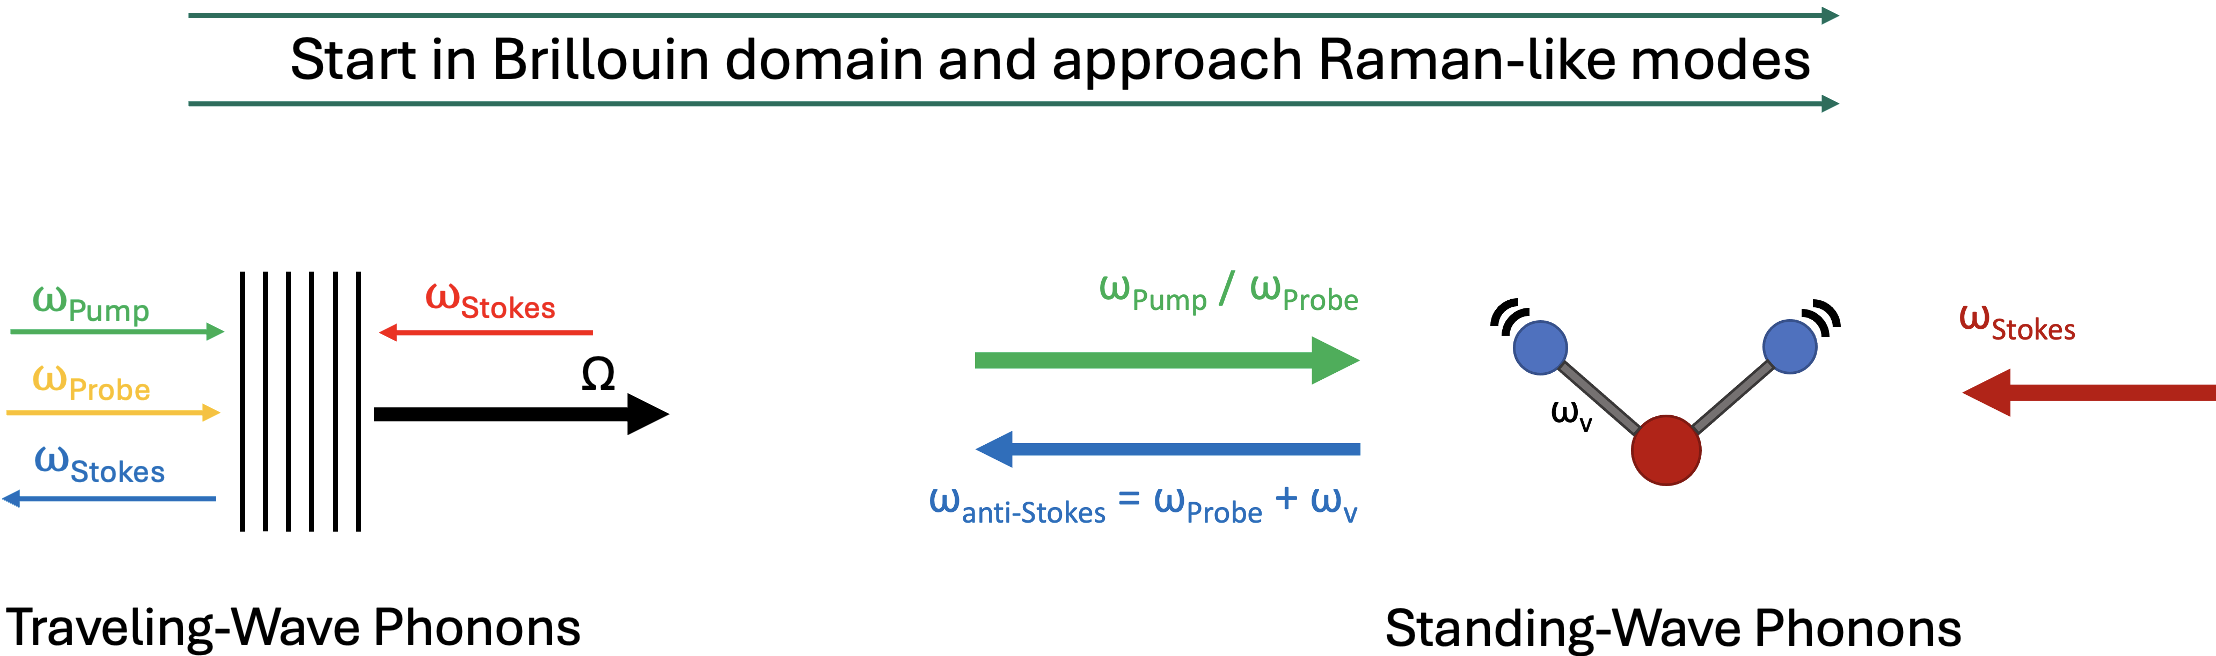
\includegraphics[width=\textwidth]{figs/4-Raman/ExploreBrillouinRamanTransition.png}
  \caption{Transition from Brillouin domain to Raman-like modes.}
  \label{fig:Raman:BrillouinRamanTransition}
\end{figure}

\begin{figure}[t]
  \centering
  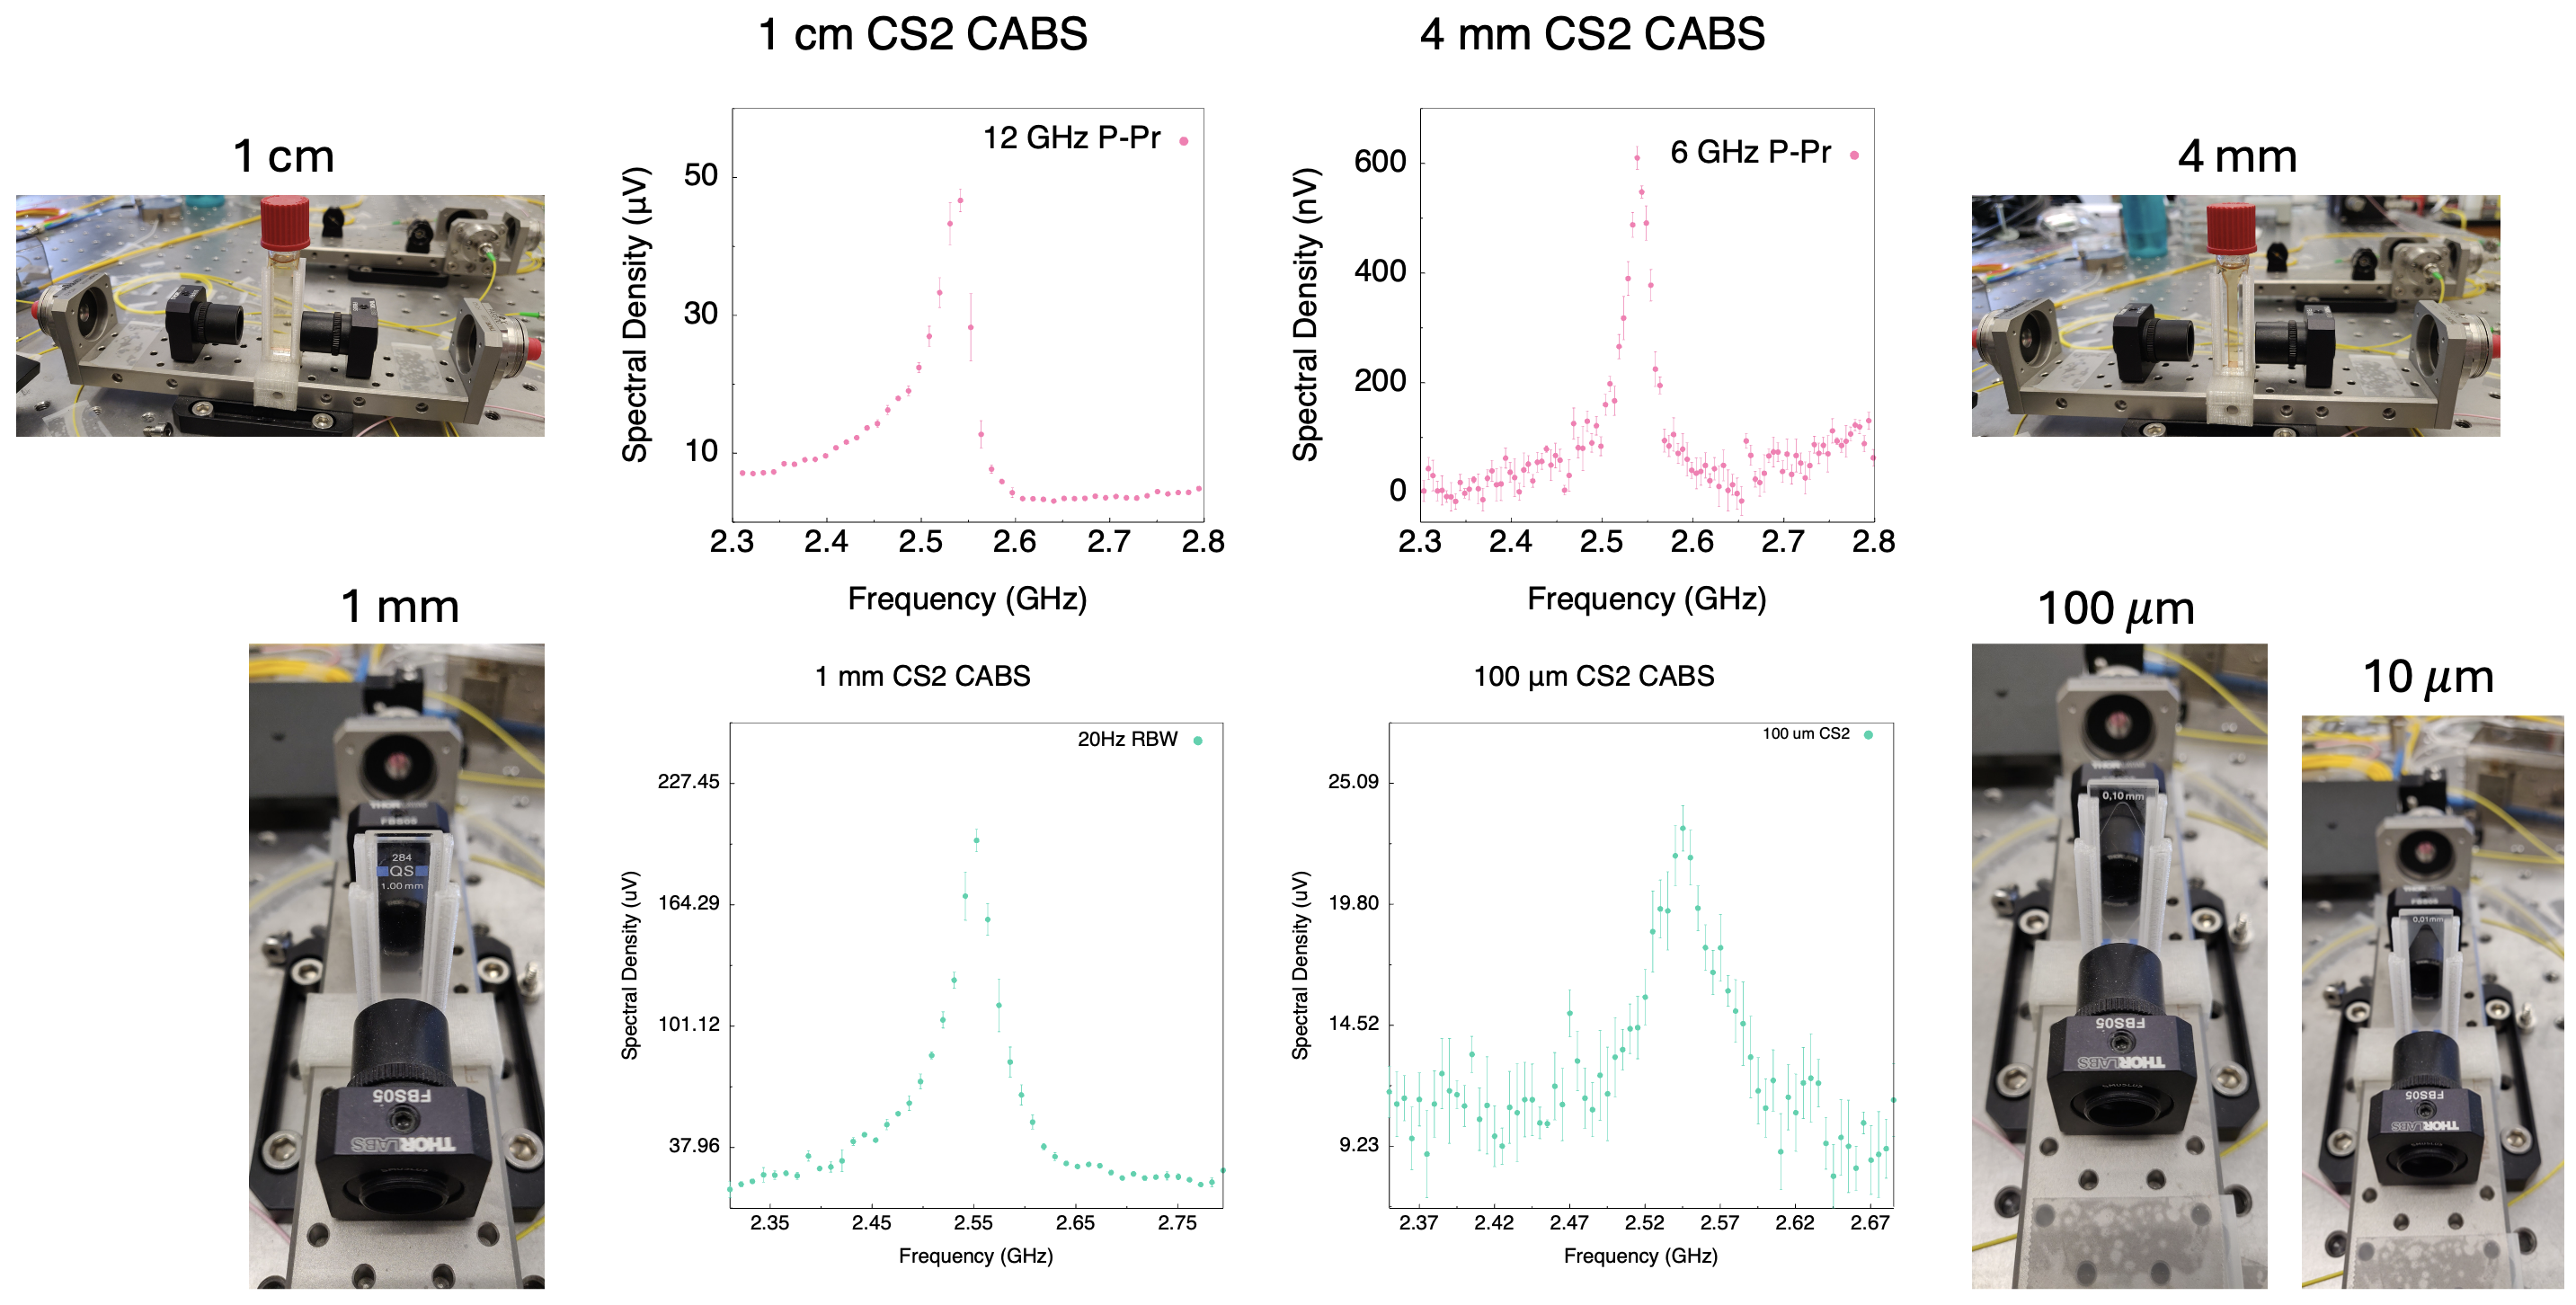
\includegraphics[width=\textwidth]{figs/4-Raman/StartBigApproachSmall.png}
  \caption{Start big, approach small.}
  \label{fig:StartBigApproachSmall}
\end{figure}

\begin{figure}[t]
  \centering
  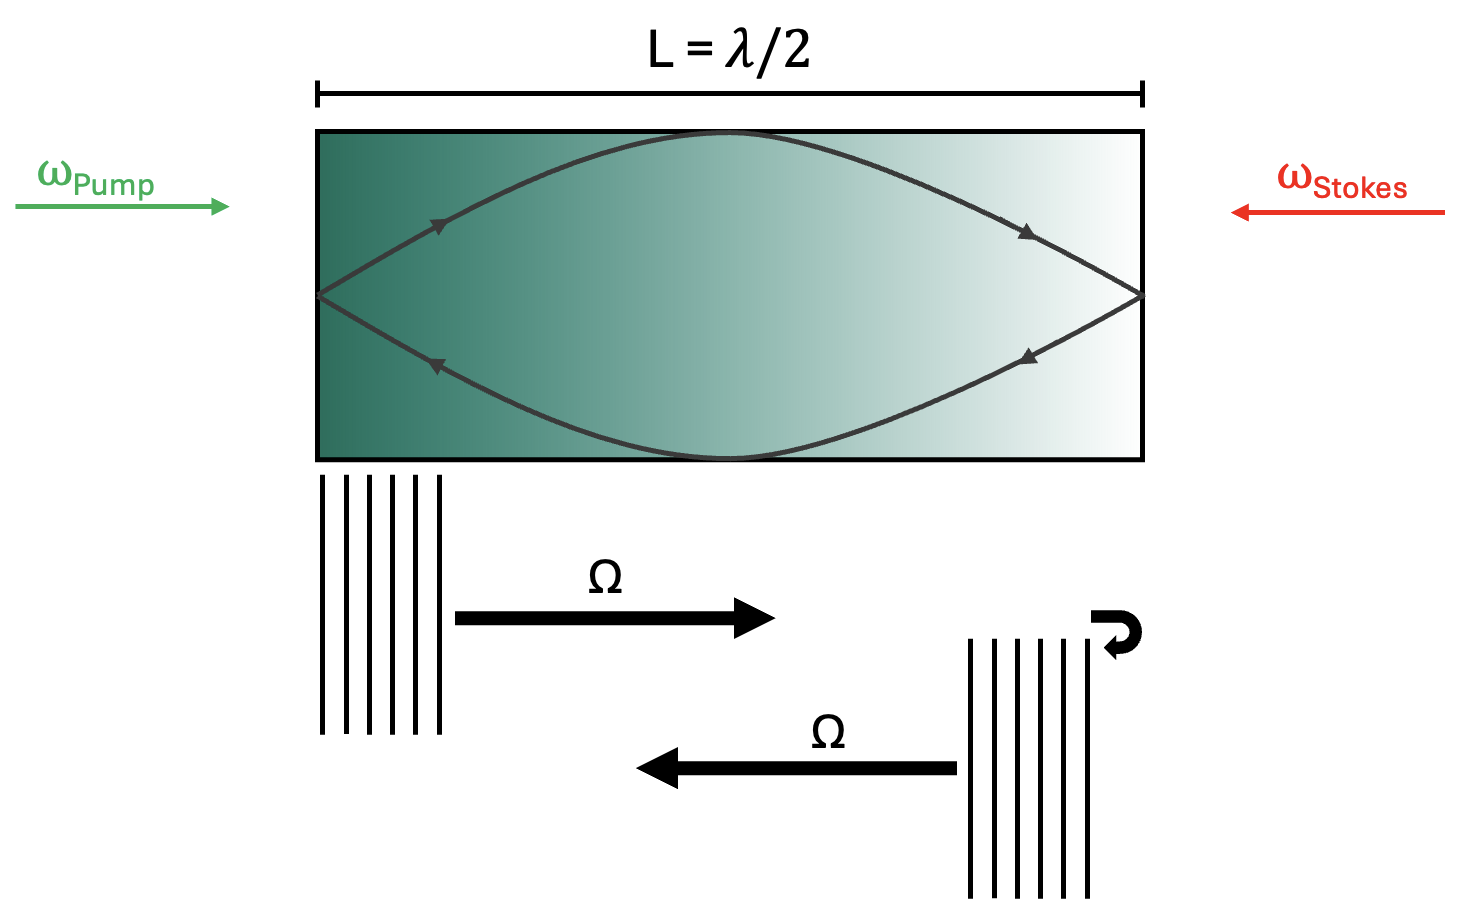
\includegraphics[width=.85\textwidth]{figs/4-Raman/GeometryDeterminesFundamentalFreq.png}
  \caption{Geometry determines fundamental frequency.}
  \label{fig:Raman:GeometryDeterminesFundamentalFreq}
\end{figure}

\subsection{Key Parameters and Feasibility}
\label{subsec:Raman:KeyParametersandFeasibility}

Observing Raman-like standing-wave modes via \ac{SBS} hinges on several key parameters of the system. We identify three especially critical factors: (1) the scattered power, determined by the effective material Brillouin gain and length as well as the optical powers; (2) the acoustic dissipation in the medium, which limits the mean phonon travel distance; and (3) the acoustic boundary reflectivity, determined by impedance mismatch at interfaces, which enables the phonons to reflect and form standing-waves. These parameters together determine whether the phonon will remain a distributed traveling excitation or collapse (blur) into discrete modes. The material’s Brillouin gain coefficient \(g_{\rm 0}\) (or overlap‐adjusted effective gain \(G_{\rm B}\)) sets how strongly the phonons are driven for given pump \(P_{\rm P}\), Stokes \(P_{\rm S}\), and probe \(P_{\rm Pr}\) optical powers over an interaction length \(L\) in the \ac{CoBS} process (see Chapter~\ref{ch:CoBS}, and specifically Equation~\ref{Eq:Theoretical Framework:Scattered Power}).  Short samples demand very high Brillouin gain to achieve significant scattered power in a small \(L\). Certain tellurium‐based materials, for instance, can offer gains orders of magnitude higher than silica, \cite{sanghera2010nonlinear, abedin2005observation} allowing measureable scattered power in sub‐\si{\milli\meter} cavities.

Even if phonons are driven strongly, they must live long enough (i.e., have a low enough dissipation rate, or high enough acoustic Q) to form a standing wave. At room temperature, intrinsic damping can limit phonon \(Q_{\rm s}\) to \(\sim 10^{3}\)–\(10^{4}\) in many solids, \cite{heiman1979brillouin, bucaro1974high} implying attenuation lengths of \si{\milli\meter} to \si{\centi\meter} for \si{\giga\hertz} frequencies. Ideally, the sample length \(L\) should be comparable to or less than half the attenuation length so that phonons undergo multiple round trips. This is considerably more difficult at room temperature than at cryogenic temperatures, where \(Q_{\rm s}\) can exceed \(10^{7}\). \cite{maris1990phonon, renninger2018bulk} Finally, the phonon must reflect rather than escape at the boundaries. A large acoustic impedance mismatch (e.g., a free surface with air on one side) can approach nearly 100\% reflection. \cite{galliou2013extremely, auld1973acoustic} Designing the sample with two opposing highly acoustically reflective boundaries is the most straightforward path to generating a Raman-like standing-wave mode in the medium. In practice, however, partial reflections at both ends can also suffice so long as the net round‐trip reflectivity is high enough to sustain a mode.

In essence, we want to create a high-\(Q\) acoustic resonator inside a Brillouin-active medium at room temperature: strong enough \ac{CoBS} driving to excite the phonons, low enough damping to maintain them, and robust boundary reflections to confine them. Meeting all of these conditions can be challenging. Nonetheless, feasibility estimates and preliminary \ac{CoBS} measurements indicate that by using ultra-high-gain media (such as \ce{Te} \cite{sanghera2010nonlinear, abedin2005observation} or liquid \ce{CS2} \cite{boyd2020nonlinear}), shortening the cavity, and ensuring a free boundary, one can push toward Brillouin-induced Raman modes even under ambient conditions. In what follows, we detail the experimental platforms, theoretical modeling, and attempts to observe discrete phonon modes in high-gain materials. Although a conclusive demonstration proved elusive in our particular setup, largely due to technical limitations and overlapping background signals, the conceptual framework is robust and continues to motivate ongoing efforts. By shrinking the acoustic path length, maximizing phonon reflectivity, and exploiting strong \ac{CoBS} gain, one can approach the regime where traveling-wave Brillouin scattering morphs into Raman-like standing-wave modes. This pursuit effectively unifies the traveling-wave and standing-wave paradigms of light-sound interaction, providing new opportunities in cavity-free phononics, resonant optomechanics, and coherent phonon devices at room temperature.

\begin{figure}[t]
  \centering
  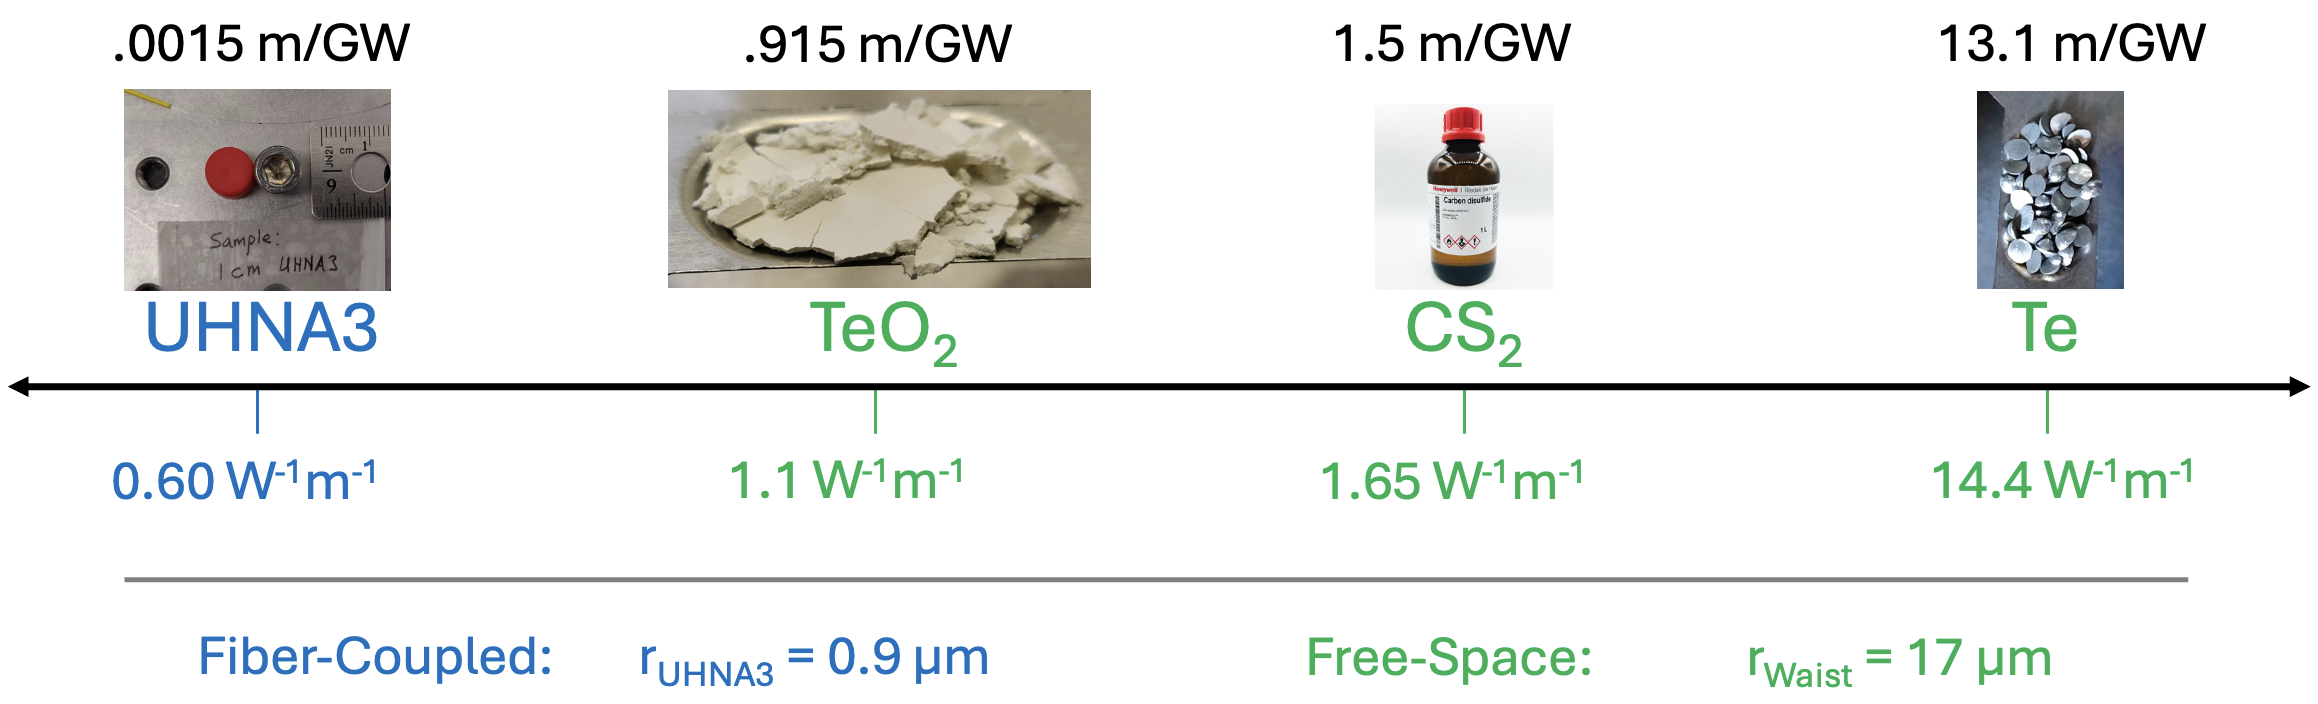
\includegraphics[width=\textwidth]{figs/4-Raman/GainOfRelevantMaterials.png}
  \caption{Gain of relevant materials.}
  \label{fig:Raman:GainOfRelevantMaterials}
\end{figure}

\begin{figure}[t]
  \centering
  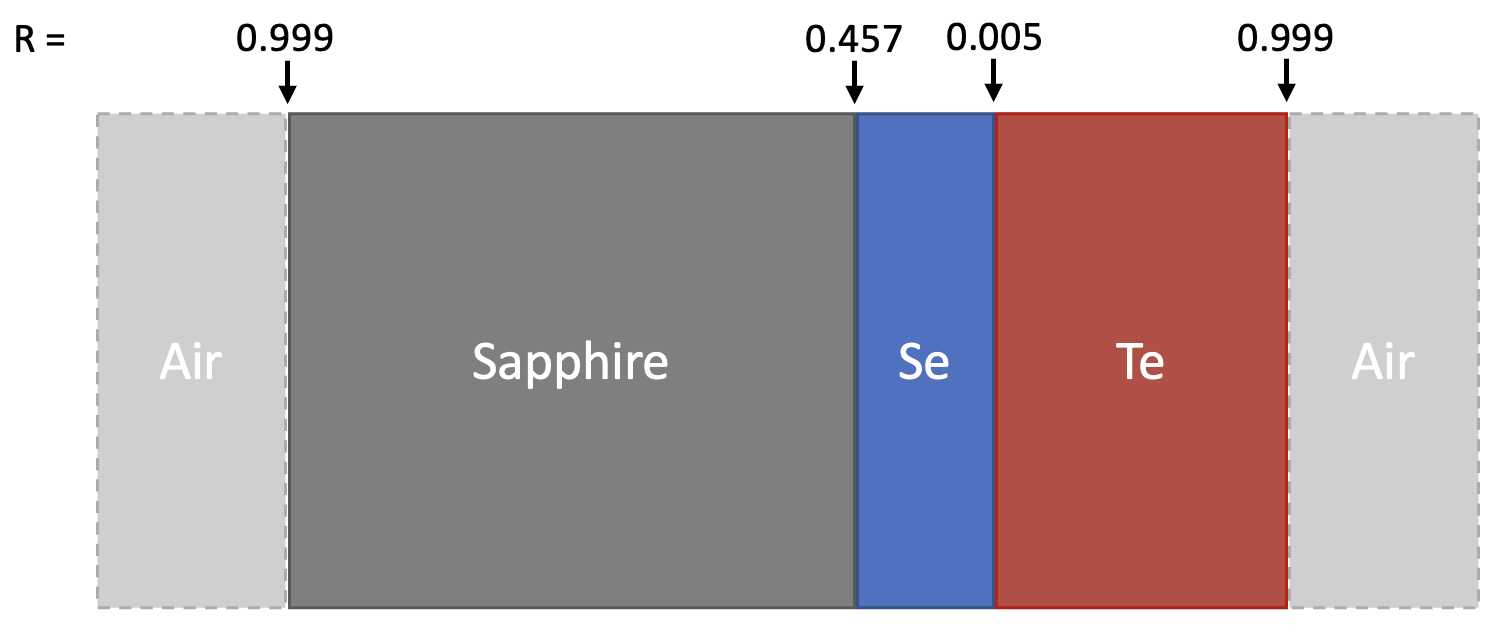
\includegraphics[width=\textwidth]{figs/4-Raman/AcousticImpedance.png}
  \caption{Acoustic impedance.}
  \label{fig:Raman:AcousticImpedance}
\end{figure}

%--------------------------------------------------------------------%

\section{Experimental Platforms and Collaborative Fabrication}
\label{sec:Raman:ExperimentalPlatformsandCollaborativeFabrication}

\subsection{Germanium-Doped Optical Fiber}
\label{subsec:Raman:Target:UHNA3}

1cm -> 1mm

\begin{figure}[t]
    \centering
    \begin{subfigure}[b]{0.49\textwidth}
        \centering
        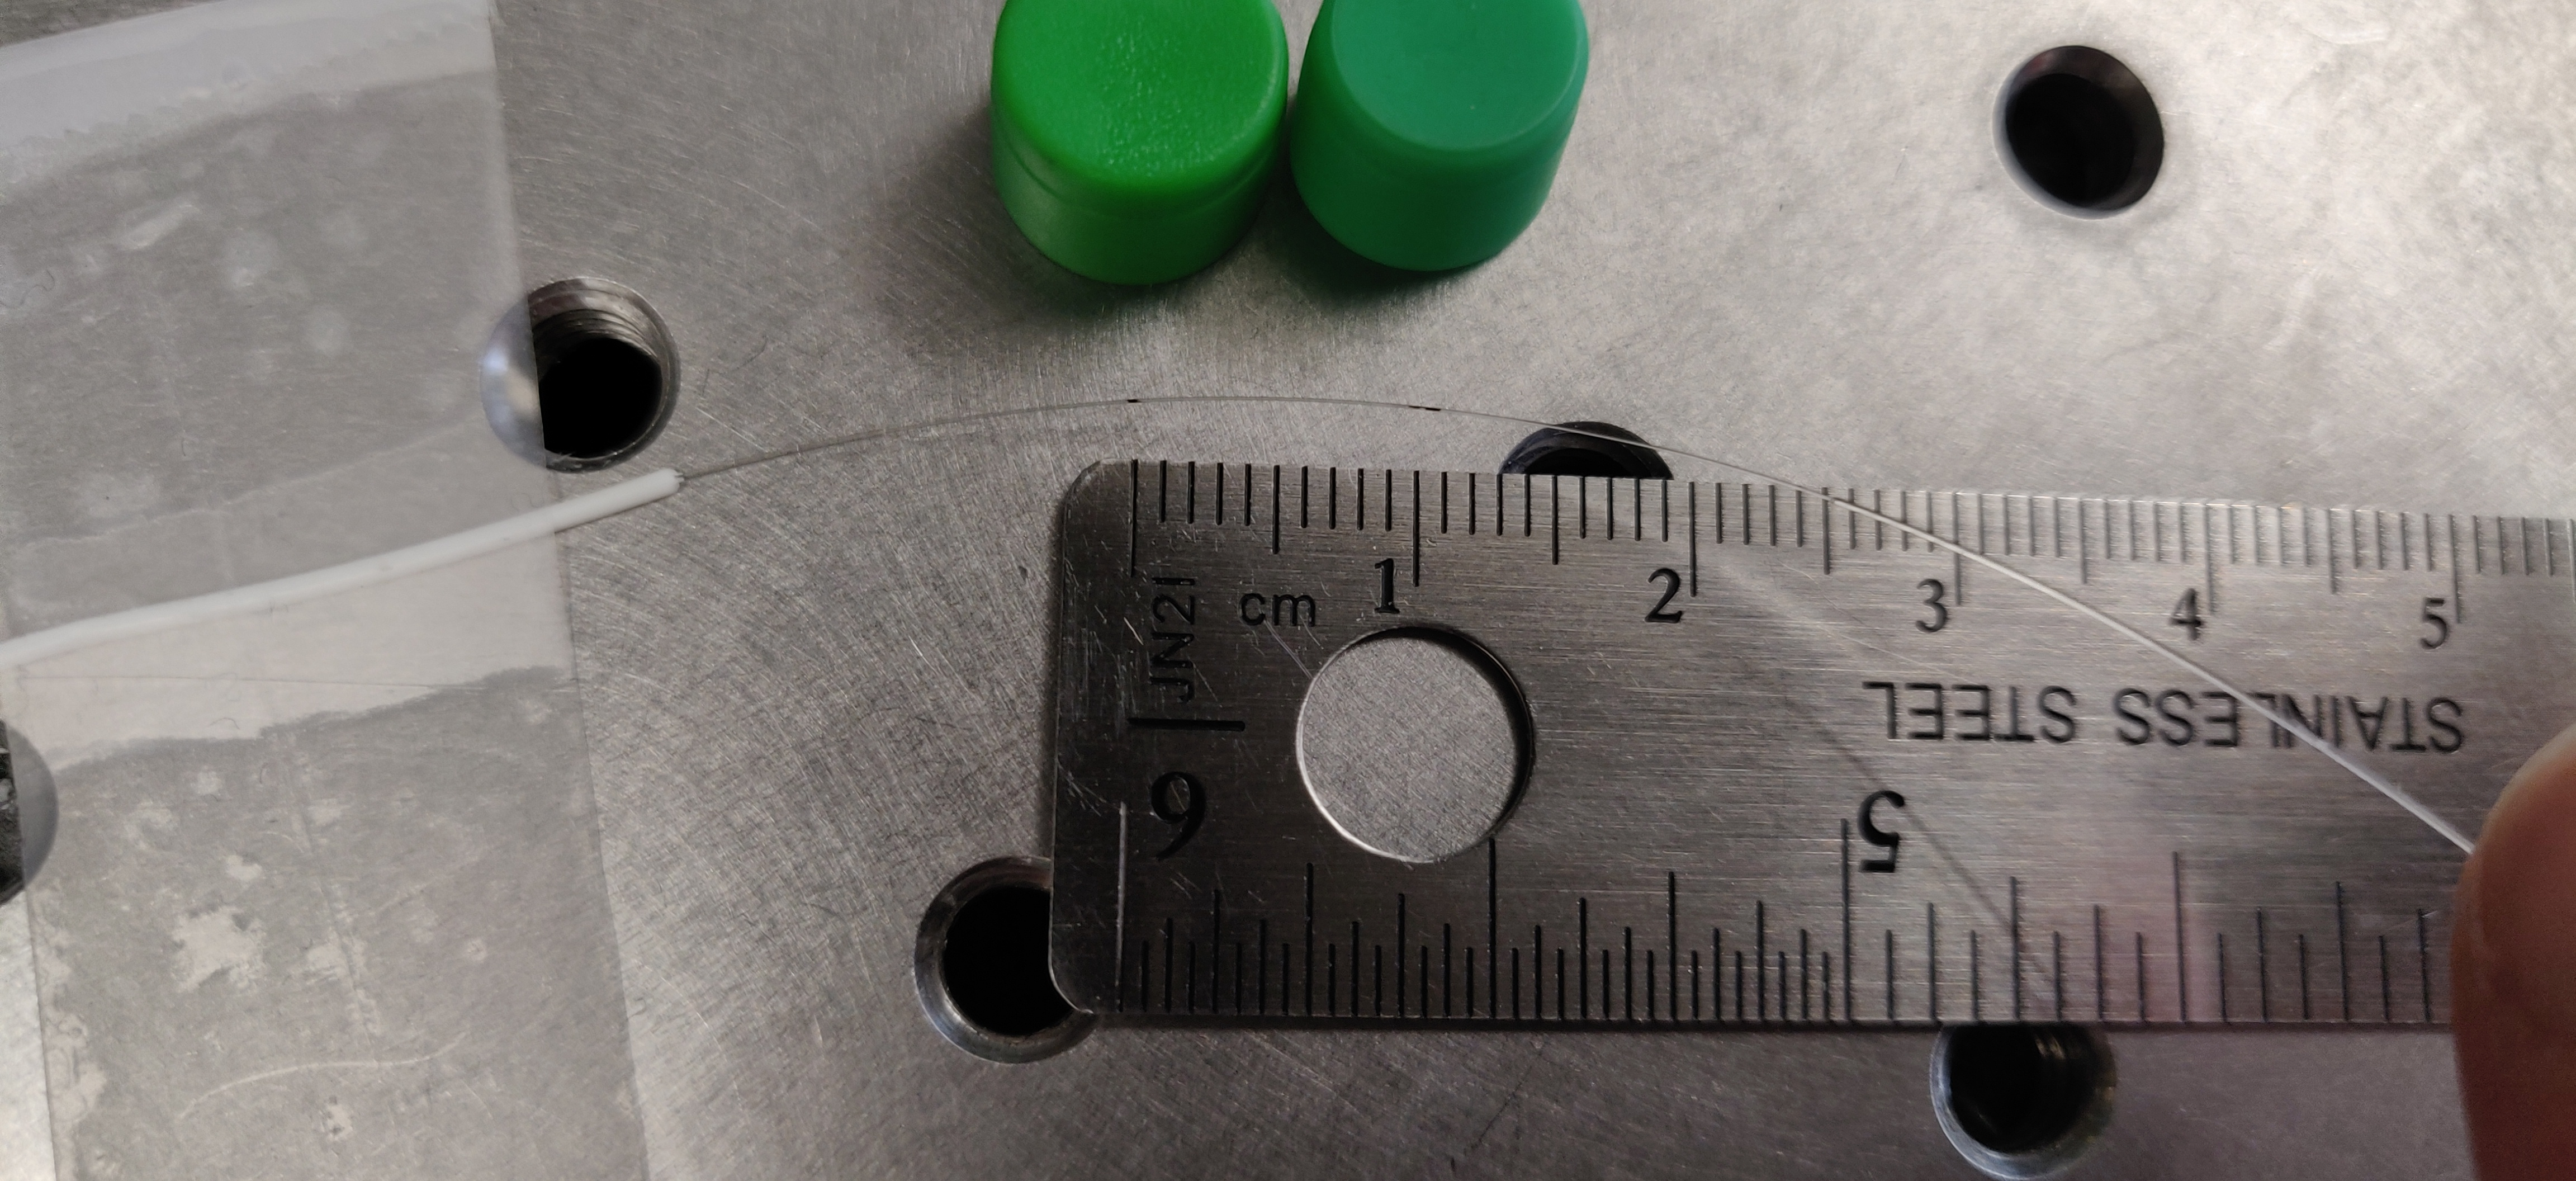
\includegraphics[width=\textwidth]{figs/4-Raman/1cm UHNA3.jpeg}
        \caption{}
        \label{fig:Raman:1cmUHNA3pic}
    \end{subfigure}
    \hfill
    \begin{subfigure}[b]{0.49\textwidth}
        \centering
        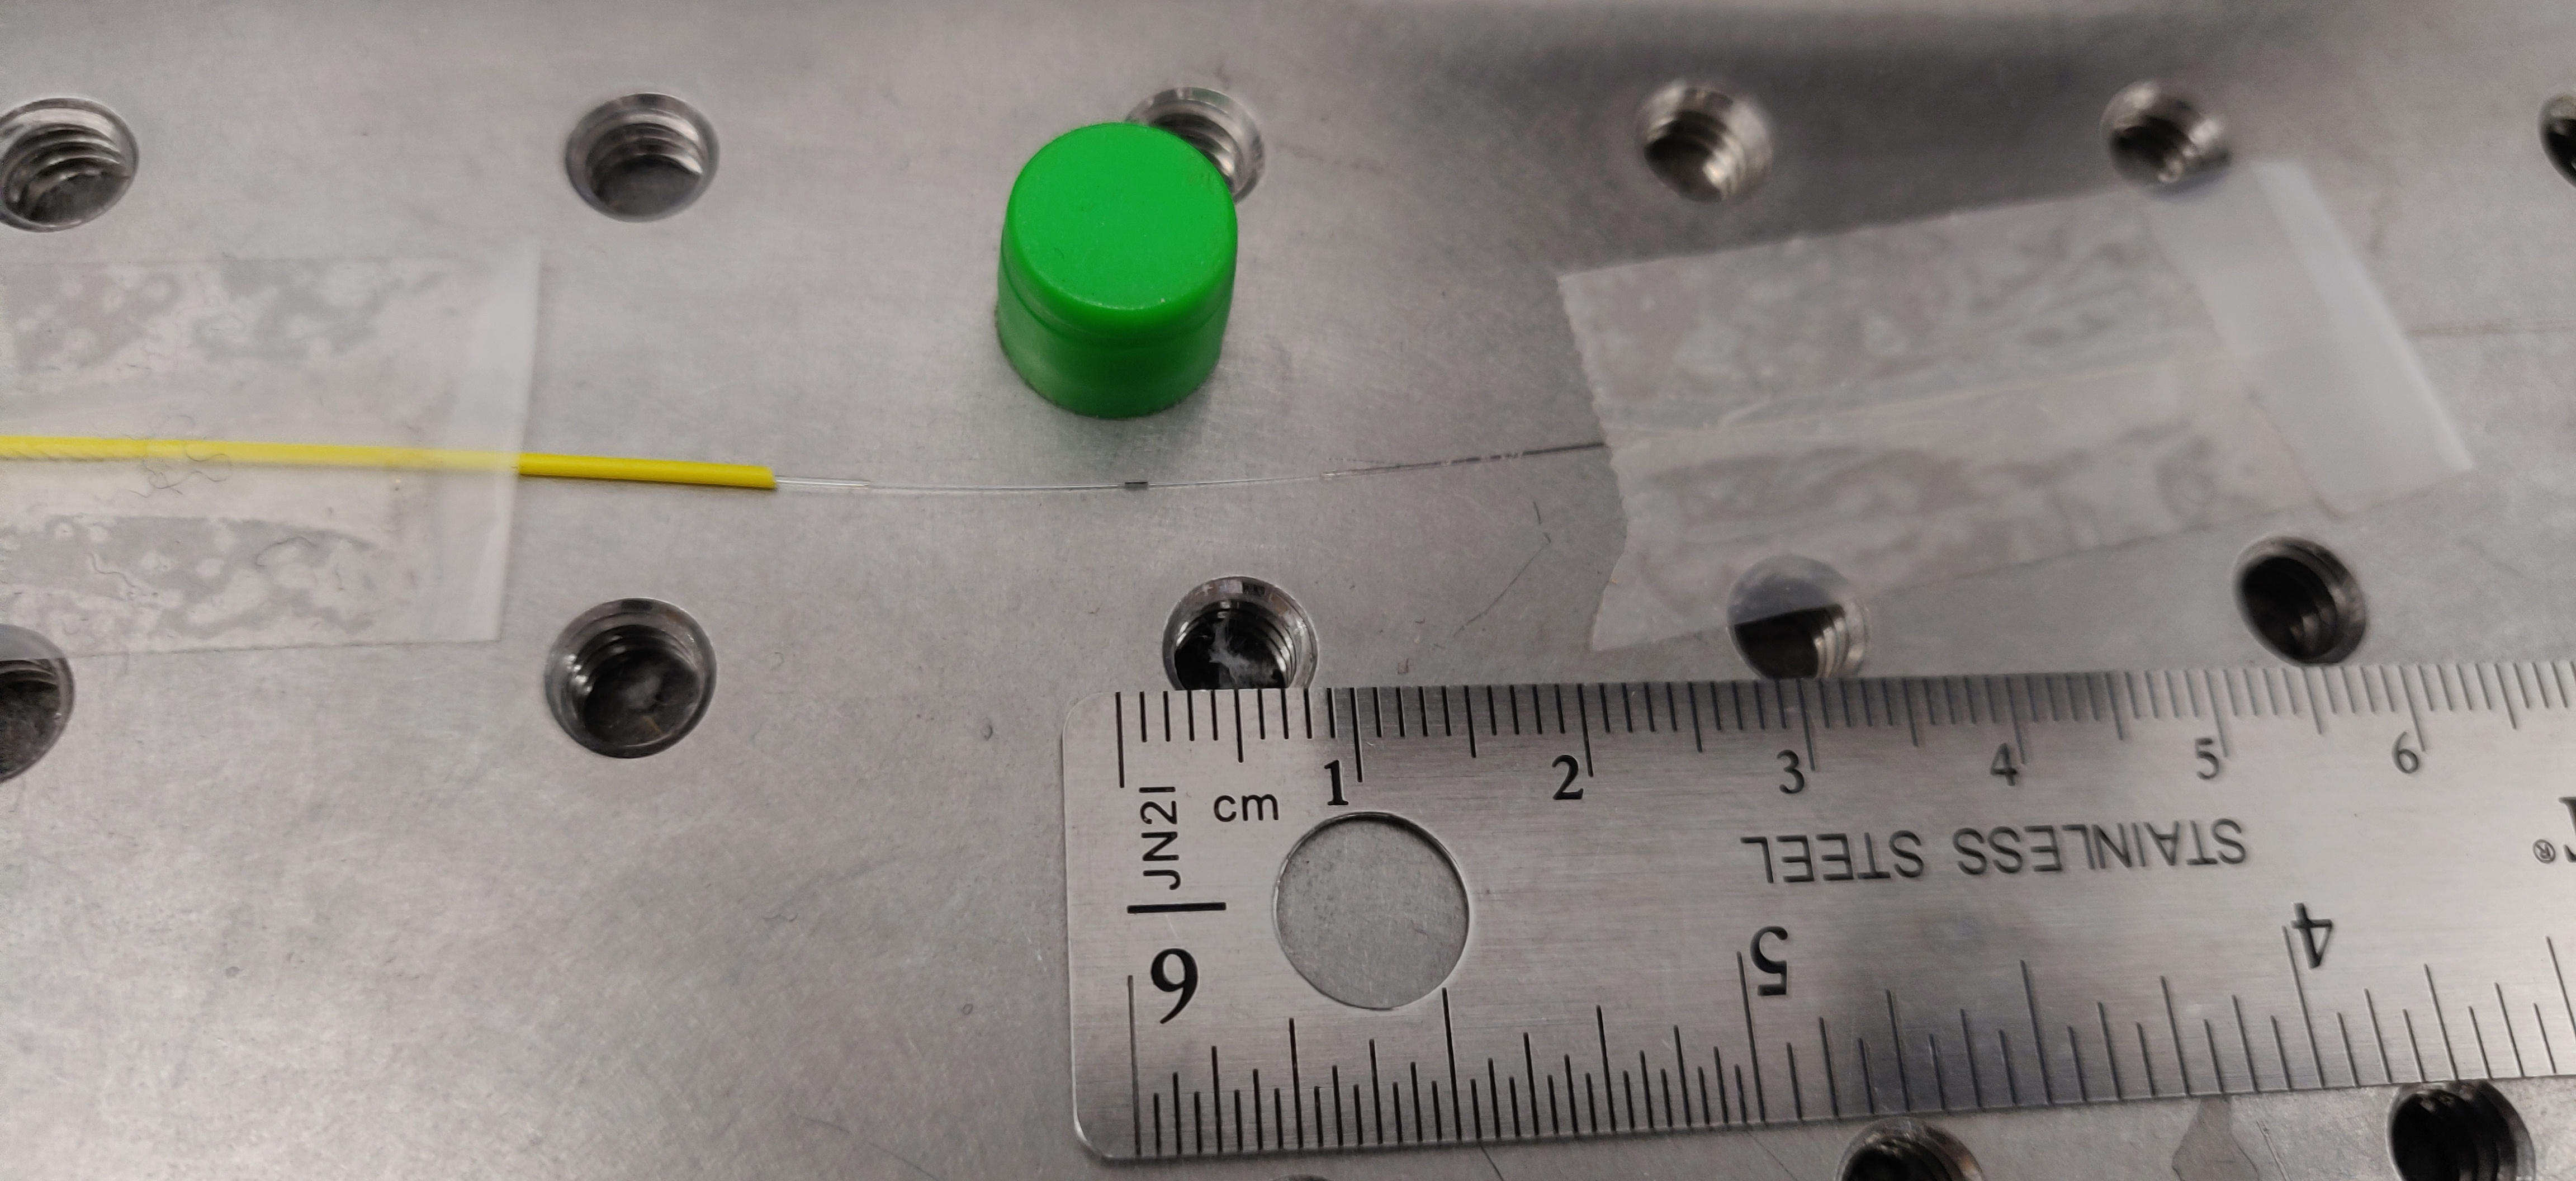
\includegraphics[width=\textwidth]{figs/4-Raman/1mm UHNA3 in apparatus.jpeg}
        \caption{}
        \label{fig:Raman:1mmUHNA3pic}
    \end{subfigure}
    \caption{\SI{1}{\centi\meter} (\ref{fig:Raman:1cmUHNA3pic}) and \SI{1}{\milli\meter} (\ref{fig:Raman:1mmUHNA3pic}) \ac{UHNA3}.}
    \label{fig:Raman:UHNA3}
\end{figure}

\subsection{Free-Space Optics with Liquid Carbon Disulfide}
\label{subsec:Raman:Target:CS2Vial}

Free space with vial

\begin{figure}[t]
    \centering
    \begin{subfigure}[b]{0.49\textwidth}
        \centering
        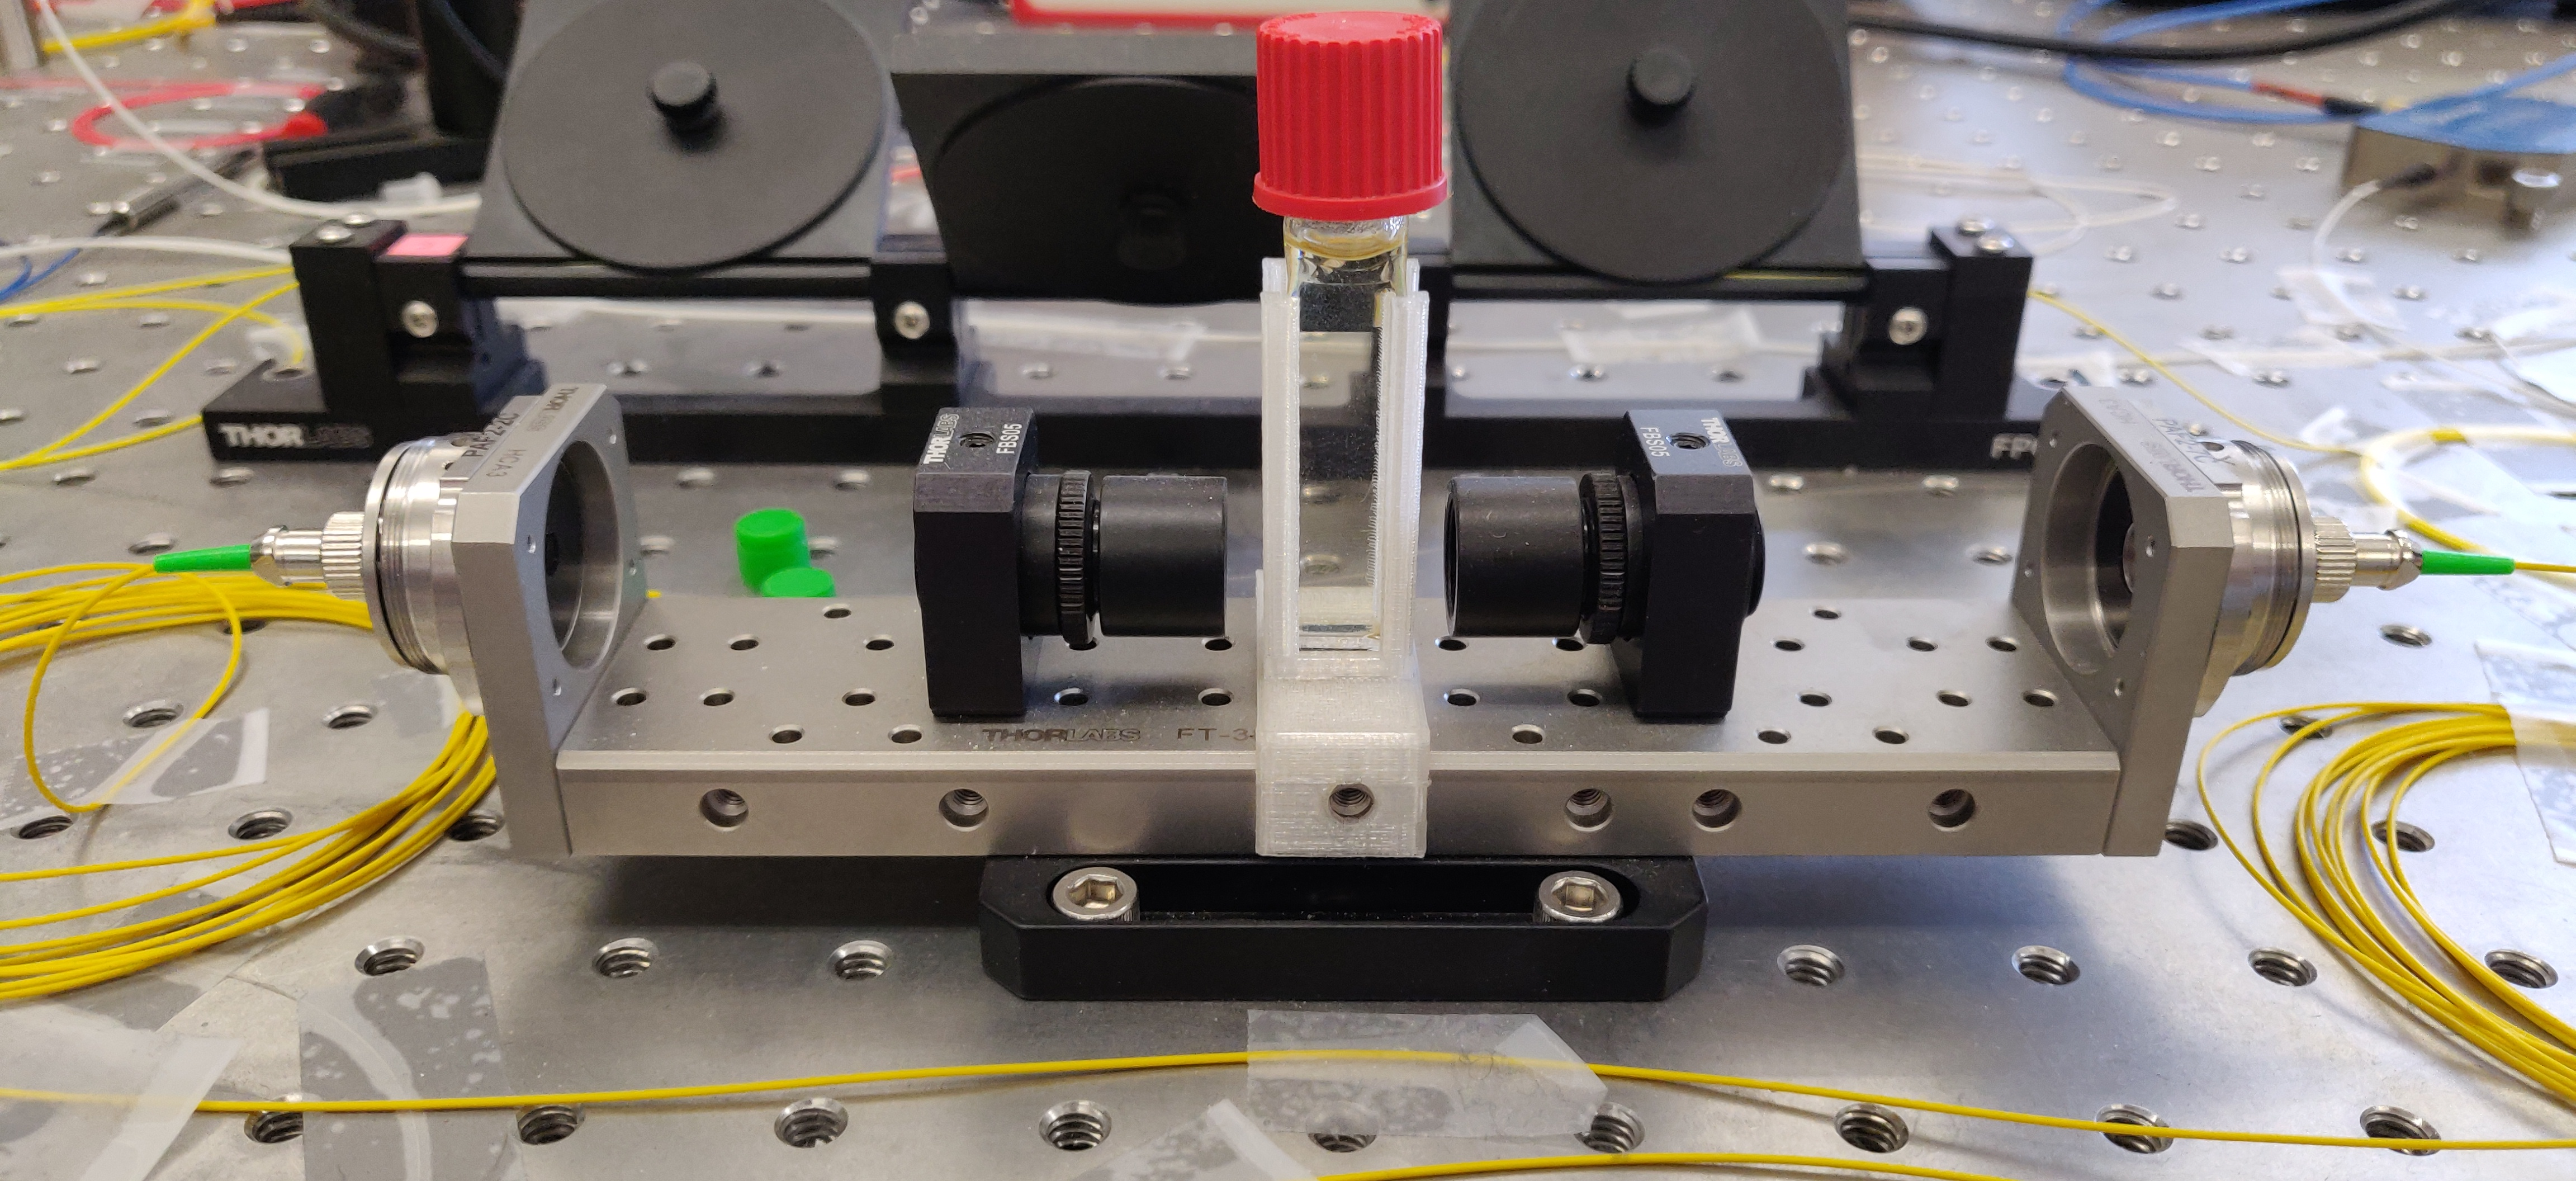
\includegraphics[width=\textwidth]{figs/4-Raman/1cmCS2.jpeg}
        \caption{}
        \label{fig:Raman:1cmCS2}
    \end{subfigure}
    \hfill
    \begin{subfigure}[b]{0.49\textwidth}
        \centering
        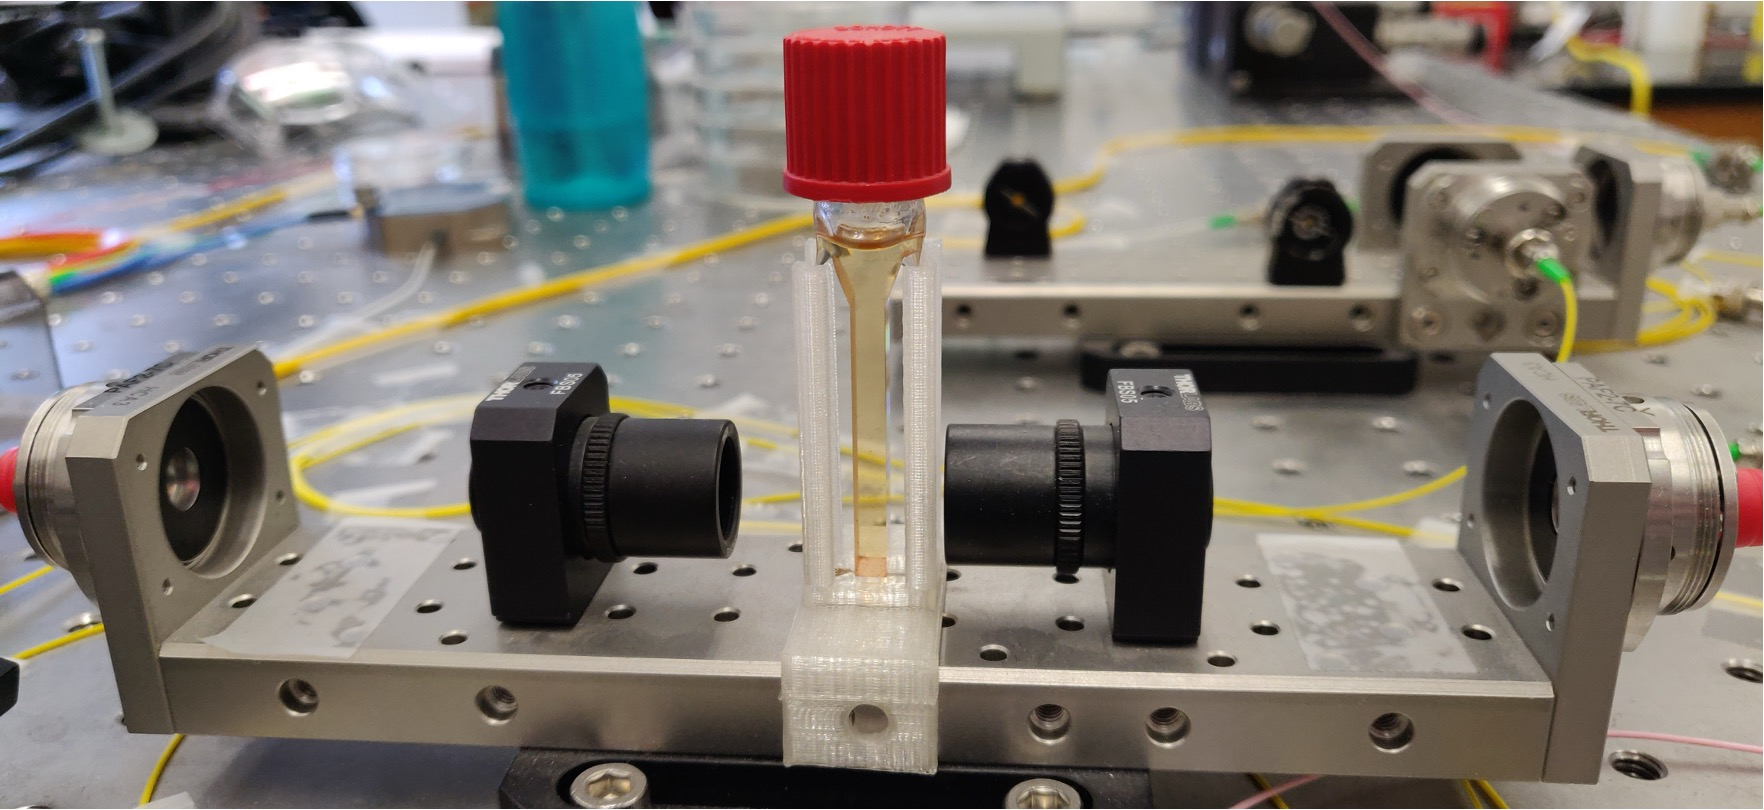
\includegraphics[width=\textwidth]{figs/4-Raman/4mmCS2.jpg}
        \caption{}
        \label{fig:Raman:4mmCS2}
    \end{subfigure}
    \caption{\SI{1}{\centi\meter} (\ref{fig:Raman:1cmCS2}) and \SI{4}{\milli\meter} (\ref{fig:Raman:4mmCS2}) liquid \ce{CS2}.}
    \label{fig:Raman:CS2Cuvet}
\end{figure}

\subsection{Tellurium Dioxide Thin Film}
\label{subsec:Raman:Target:TeO2}

Gibbs collab
deposit Te, oxidize into TeO2

table of relevant TeO2 parameters

\subsection{Tellurium Thin Film}
\label{subsec:Raman:Target:Te}

Gibbs collab and CINT collab
oxidizes to TeO2

table of relevant Te parameters

\subsection{Carbon Disulfide Micrometer Cell}
\label{subsec:Raman:Target:CS2Cells}

table of relevant CS2 parameters

cells -> 1 W amp, bubble test

\begin{figure}[t]
  \centering
  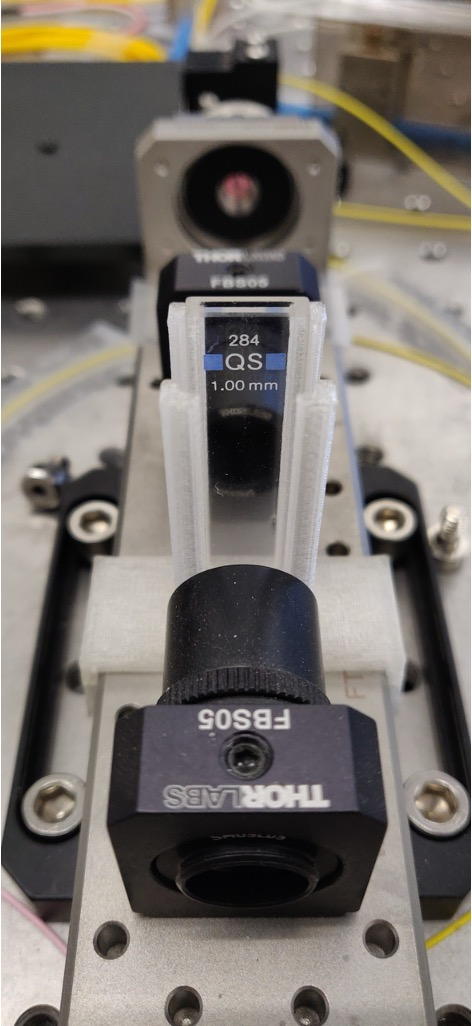
\includegraphics[height=.8\textheight]{figs/4-Raman/1mmCS2.jpg}
  \caption{\SI{1}{\milli\meter} \ce{CS2} cell secured in beam path of \acl{CoBS}.}
  \label{fig:Raman:1mmCS2}
\end{figure}

\begin{figure}[t]
  \centering
  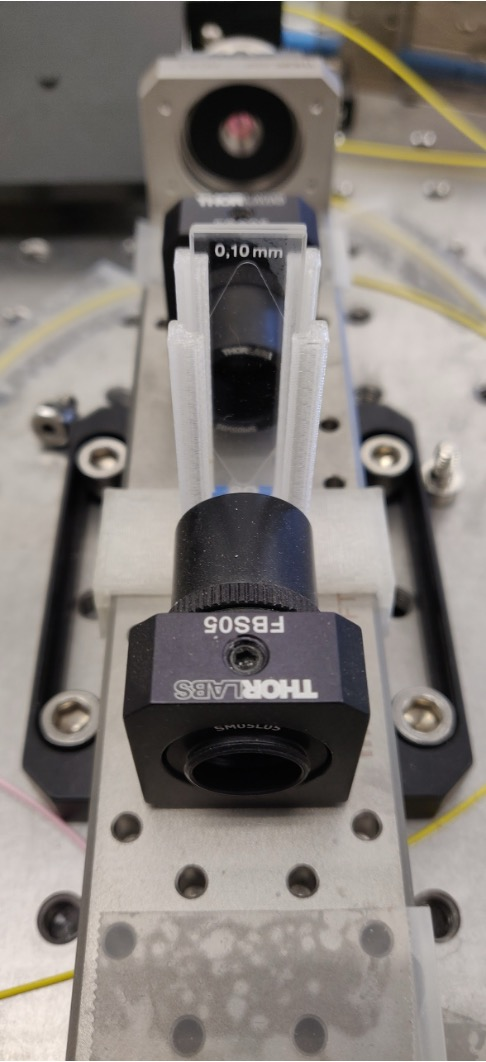
\includegraphics[height=.8\textheight]{figs/4-Raman/100umCS2.jpg}
  \caption{\SI{100}{\micro\meter} \ce{CS2} cell secured in beam path of \acl{CoBS}.}
  \label{fig:Raman:100umCS2}
\end{figure}

\begin{figure}[t]
  \centering
  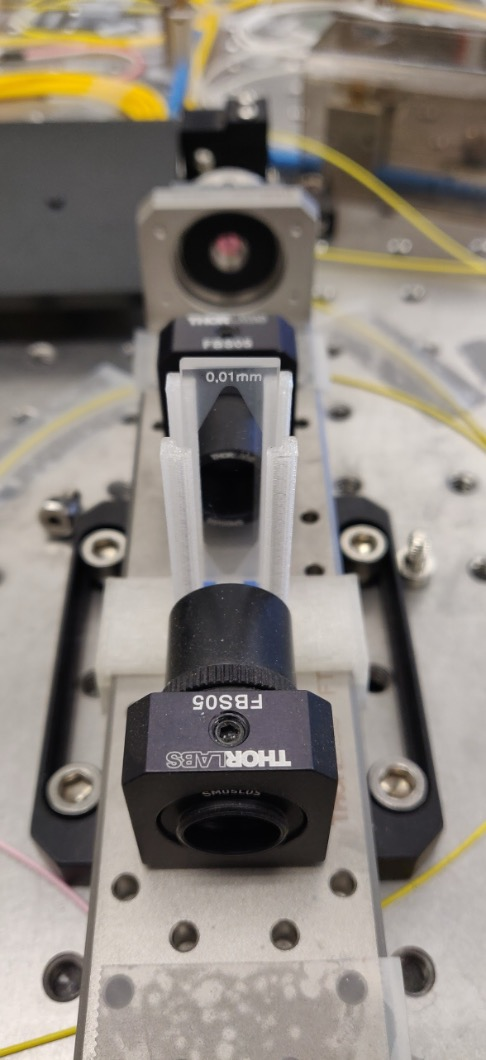
\includegraphics[height=.8\textheight]{figs/4-Raman/10umCS2.jpg}
  \caption{\SI{10}{\micro\meter} \ce{CS2} cell secured in beam path of \acl{CoBS}.}
  \label{fig:Raman:10umCS2}
\end{figure}

\subsection{Suspended Silica Rib Waveguide}
\label{subsec:Raman:Target:Waveguide}

BYU collab
If we can couple chip waveguide into CoBS fiber-chip-fiber, then we have access to a playground of materials and geometries
initial test took 9 months to learn and measure


\subsection{Elastically-Suspended Photonic-Phononic Waveguide}
\label{subsec:Raman:Target:WigglyWaveguide}

BYU collab
proof of fabrication: holes and trampoline

%--------------------------------------------------------------------%

\section{Methods}
\label{sec:Raman:Methods}

\subsection{Instrument Overview}
\label{subsec:Raman:InstrumentOverview}

\begin{itemize}
  \item Recap the Coherently Stimulated Brillouin Spectrometer from Chapter 3, emphasizing its high sensitivity and relaxed phase-matching.
  \item Note additional improvements or calibration steps performed for these particular experiments.
\end{itemize}

\subsection{Measurement Protocol}
\label{subsec:Raman:MeasurementProtocol}

\begin{itemize}
  \item Walk through how pump and probe fields are injected into the samples (liquid cells, waveguides, films).
  \item How you monitor and collect scattered light at/near the expected Brillouin frequency, watching for discrete or multi-peak features.
  \item Typical data-acquisition settings (power ranges, frequency scans, detection bandwidth, etc.).
\end{itemize}

\subsection{Data Analysis Steps}
\label{subsec:Raman:DataAnalysisSteps}

\begin{itemize}
  \item Call back to Lorentzian versus Fano-shape fitting for small signals
  \item Mention Lorentzian versus multi-peak fitting to identify discrete modes.
  \item Emphasize strategies to distinguish genuine signals from instrument background, referencing instrument artifacts discovered previously.
  \item Summarize how you accounted for temperature effects, boundary reflections, or chemical transformations (like Te to TeO\textsubscript{2}).
\end{itemize}

%--------------------------------------------------------------------%

\section{Results}
\label{sec:Raman:Results}

UHNA3 - 1cm, 1mm
CS2 vial - 4mm, 2mm
TeO2 films - 1um, 500nm
CS2 - 1mm, 100um, (10um not quite)
chip waveguide - chip/nochip, holes

\subsection{Initial Findings}
\label{subsec:Raman:InitialFindings}

\begin{itemize}
  \item Display earliest data (e.g., on Te thin films) and how a strong feature turned out to be electronic background.
  \item Show subsequent measurements (CS\textsubscript{2}, chip waveguides) and partial successes, such as spectral distortions suggesting mode splitting.
\end{itemize}

\subsection{Challenges and Partial Outcomes}
\label{subsec:Raman:ChallengesandPartialOutcomes}

\begin{itemize}
  \item Explain complexity of proving Raman-like modes: acoustic mismatch, unexpected phonon damping, oxidation/ablation of thin films, or sample delays.
  \item Highlight any improvements you achieved (e.g., 11\(\times\) scattered-signal boost) and how close you were to threshold detection.
\end{itemize}

\subsection{Interpretation in Light of Theory}
\label{subsec:Raman:InterpretationinLightofTheory}

\begin{itemize}
  \item Note which observations align with the traveling-wave to standing-wave hypothesis.
  \item Speculate on why a clear discrete Raman ladder was not definitively observed (path length, reflectivity, line broadening, etc.).
\end{itemize}

\begin{figure}[t]
  \centering
  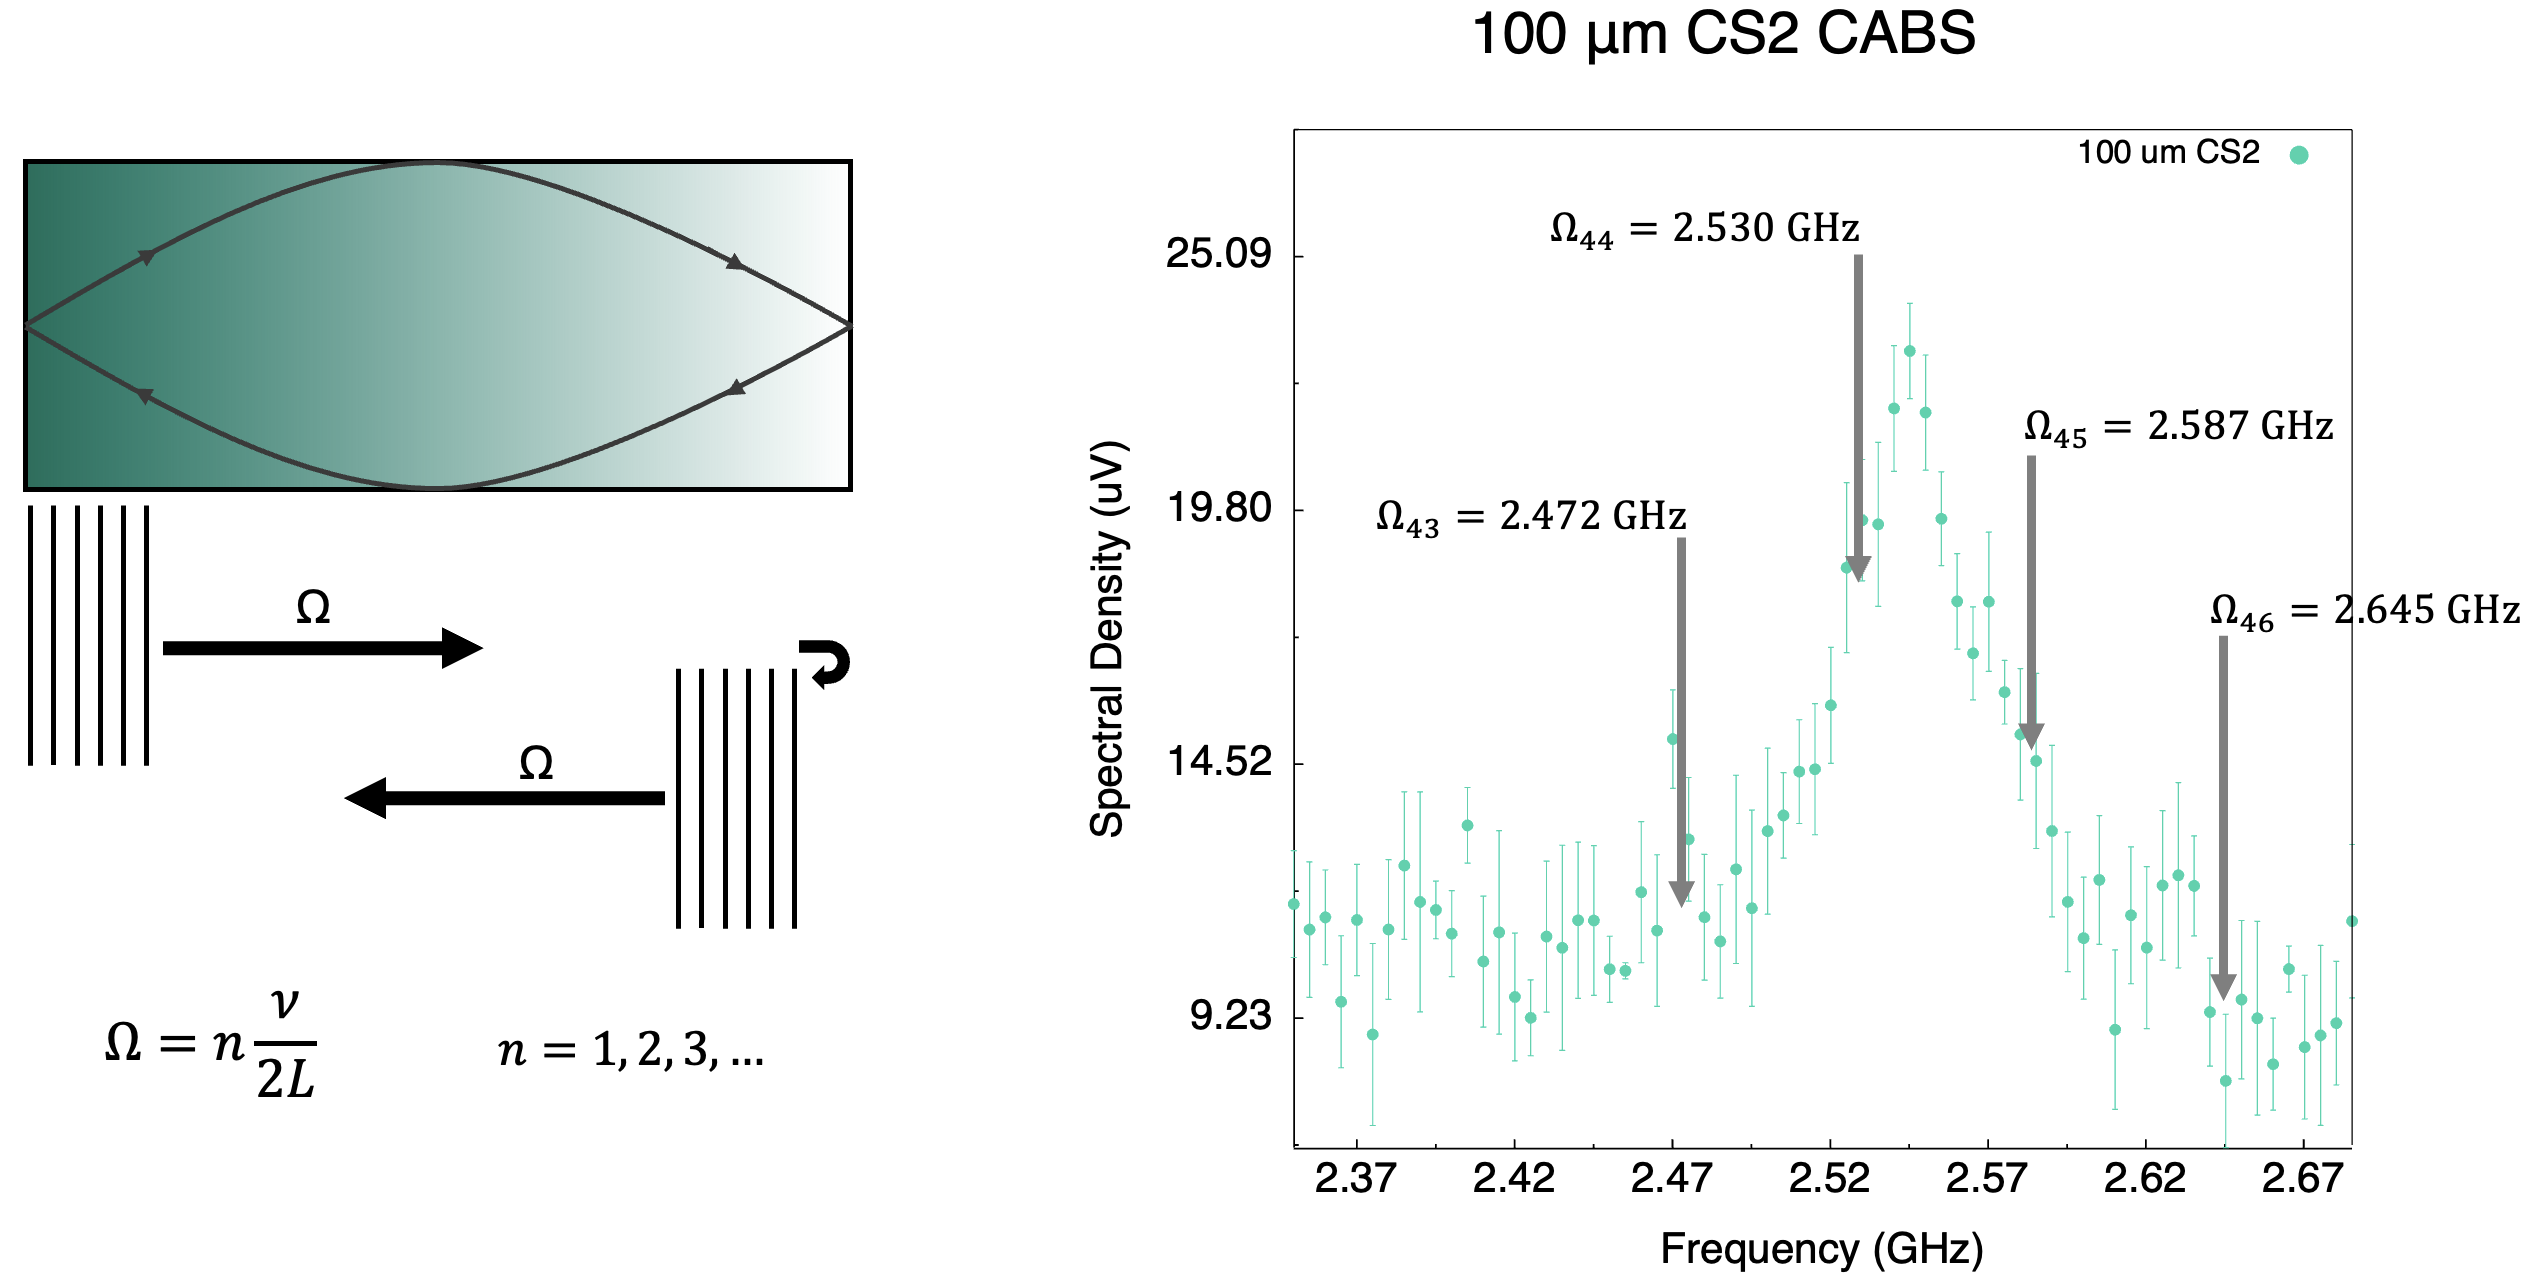
\includegraphics[width=\textwidth]{figs/4-Raman/HowWouldRamanModesAppear.png}
  \caption{How would Raman modes appear.}
  \label{fig:HowWouldRamanModesAppear}
\end{figure}

%--------------------------------------------------------------------%

\section{Discussion}
\label{sec:Raman:Discussion}

\subsection{Pathways to Brillouin-Induced Raman Modes}
\label{subsec:Raman:Pathways}
Ideal platforms by category
  waveguide - long TeO2 rib, evenly spaced square holes
  TeO2 thin film/crystal - dissolve only small area of substrate for beam spot
  CS2 cell - 5um
  Fiber - notched, acoustic fiber Bragg grating

\subsection{Conclusion}
\label{subsec:Raman:Conclusion}

\begin{itemize}
\item \textbf{Connection to Dissertation Theme}
  \begin{itemize}
    \item Relate back to the broader aims of controlling phonons at room temperature, highlighting how these efforts extend your dissertation’s exploration of optomechanical interactions.
  \end{itemize}
\end{itemize}

\clearpage
\thispagestyle{empty}
\null
\newpage
